\documentclass[conference]{IEEEtran}
\IEEEoverridecommandlockouts
\usepackage{cite}
\usepackage{amsmath,amssymb,amsfonts}
\usepackage{algorithmic}
\usepackage{algorithm}
\usepackage{graphicx}
\usepackage{textcomp}
\usepackage{xcolor}
\usepackage{booktabs}
\usepackage{multirow}
\usepackage{url}
\usepackage{balance}

\def\BibTeX{{\rm B\kern-.05em{\sc i\kern-.025em b}\kern-.08em
    T\kern-.1667em\lower.7ex\hbox{E}\kern-.125emX}}

\begin{document}

\title{Threat Evolution Modeling for Online and Offline Cybersecurity Monitoring Using Behavioral Digital Twins and Temporal Knowledge Graphs}

\author{
  \makebox[\textwidth][c]{
    \begin{minipage}{0.65\textwidth}
      \centering
      Rajesh Arepalli\\
      \textit{M.Tech. (Ph.D.), Senior Assistant Professor}\\
      \textit{Sri Vasavi Engineering College}\\
      Tadepalligudem, India
    \end{minipage}
  }\\[1.5em]
  \makebox[\textwidth][c]{
    \begin{minipage}{0.48\textwidth}
      \centering
      Pujitha Paluri\\
      \textit{Computer Science and Artificial Intelligence}\\
      \textit{Sri Vasavi Engineering College}\\
      Tadepalligudem, India
    \end{minipage}
    \hfill
    \begin{minipage}{0.48\textwidth}
      \centering
      Sri Ranjitha Bandaru\\
      \textit{Computer Science and Artificial Intelligence}\\
      \textit{Sri Vasavi Engineering College}\\
      Tadepalligudem, India
    \end{minipage}
  }\\[1.5em]
  \makebox[\textwidth][c]{
    \begin{minipage}{0.48\textwidth}
      \centering
      Devendra Sagar Ibba\\
      \textit{Computer Science and Artificial Intelligence}\\
      \textit{Sri Vasavi Engineering College}\\
      Tadepalligudem, India
    \end{minipage}
    \hfill
    \begin{minipage}{0.48\textwidth}
      \centering
      Ajay Kumar Mandapati\\
      \textit{Computer Science and Artificial Intelligence}\\
      \textit{Sri Vasavi Engineering College}\\
      Tadepalligudem, India
    \end{minipage}
  }
}

\maketitle

\begin{abstract}
Detecting cyber threats on modern enterprise computers has become very difficult for three practical reasons. First, security operation centers are bombarded with thousands of disconnected alerts every day, causing security analysts to suffer from severe alert fatigue. Second, most intrusion detection systems treat system events as isolated data points, completely ignoring the normal daily work habits of the specific employee using the computer. Third, when employees travel or work offline without internet access, conventional cloud-based security tools stop collecting data, creating dangerous blind spots where malware can run undetected. 

To solve these practical issues, we developed \textbf{CyberZen}, an end-to-end host security monitoring system. CyberZen builds a \textit{Behavioral Digital Twin} that learns how a user normally works, such as their regular login times, the programs they usually open, and the devices they normally plug in. It uses this baseline to calculate a behavioral drift score $B(t)$. At the same time, it uses an Isolation Forest machine learning model to compute an anomaly score $A(t)$ on incoming system activities. These scores are combined with historical risk $H(t)$ into a single composite risk score: $R(t) = 0.4 A(t) + 0.4 B(t) + 0.2 H(t)$. 

To stop alert fatigue, CyberZen connects related events into a \textit{Temporal Knowledge Graph} so that multiple suspicious steps are combined into one clear incident storyline. For offline protection, CyberZen saves all events into a local SQLite queue with unique transaction IDs. Once the computer reconnects to the network, it synchronizes everything without losing data or creating duplicates. We tested CyberZen on the real-world BETH dataset (containing 763,144 records), the CIC-IDS-2017 dataset, and real Blind Eagle (APT-C-36) attack logs. CyberZen achieved a 99.92\% precision rate, reduced alert fatigue by more than 80\%, prevented 100\% of event loss during network cutoffs, and processed each event in less than one millisecond ($183.4\,\mu\text{s}$).
\end{abstract}

\begin{IEEEkeywords}
Intrusion Detection, Behavioral Digital Twin, Temporal Knowledge Graph, Isolation Forest, Threat Evolution Modeling, Offline Resilience, Advanced Persistent Threats (APT).
\end{IEEEkeywords}

\section{Introduction}
Modern organizations depend heavily on desktop computers and laptops to run everyday business operations. However, keeping these computers safe from cyber attacks has become a massive headache for security teams. In a typical corporate environment, security monitoring tools generate thousands of warning notifications every single day. Most of these notifications turn out to be harmless false alarms, such as an employee running a routine software update or downloading a large company document. Because human analysts cannot manually investigate thousands of alerts each morning, dangerous attacks often slip through completely unnoticed. This practical challenge is widely known in the industry as security alert fatigue \cite{forrest2008evolution, garcia2009anomaly}.

The biggest reason traditional security tools produce so many false alarms is that they look at events in total isolation. Traditional antivirus software and rule-based intrusion detection systems look for fixed patterns or hardcoded thresholds. For example, if a tool sees PowerShell executing a script, it might immediately raise an alert. But in real life, context matters. If an IT network administrator runs PowerShell at 11:00 AM on their primary desktop to restart a print spooler, that is normal daily business. On the other hand, if an accounting intern's computer suddenly runs PowerShell at 3:30 AM to download an unknown script from an untrusted IP address, that is almost certainly an attack. Without knowing the normal routine of the person sitting at the keyboard, security systems cannot tell the difference between normal work variations and genuine intrusions \cite{kruegel2003host, yeung2002host}.

Another serious gap in modern enterprise security is the problem of offline laptops. Today, employees frequently work while traveling, on trains, in flights, or from remote locations with unstable internet connections. Most modern Endpoint Detection and Response (EDR) platforms depend on a continuous connection to cloud servers to analyze logs. When an endpoint loses network access, the cloud agent stops receiving telemetry. Attackers are fully aware of this weakness and deliberately stage attacks, run privilege escalation scripts, and collect internal passwords while the target computer is offline \cite{han2016pidas}. Once the machine reconnects, the audit trail is often fragmented or partially overwritten.

To tackle these practical problems, we designed and built \textbf{CyberZen}. CyberZen is an intelligent, host-based threat monitoring and incident reconstruction system. It combines local machine learning with user habit profiling and temporal graph analysis. Specifically, this paper makes the following practical contributions:
\begin{enumerate}
    \item \textbf{A Practical Behavioral Digital Twin}: We construct a lightweight profile for every user and computer. This profile tracks normal working hours, commonly used applications, trusted hardware devices, and average network traffic. CyberZen calculates a numerical behavioral drift score $B(t)$ whenever incoming activity deviates from these established habits.
    \item \textbf{A Balanced Threat Evolution Formula}: We combine statistical machine learning anomalies $A(t)$, behavioral drift $B(t)$, and historical risk decay $H(t)$ into a single composite equation: $R(t) = 0.4 A(t) + 0.4 B(t) + 0.2 H(t)$. This multi-factor approach prevents isolated spikes from triggering false alarms while ensuring persistent attacks accumulate high risk over time.
    \item \textbf{Temporal Knowledge Graph for Incident Reconstruction}: Instead of showing twenty separate warning popups for twenty small actions, CyberZen links related events using a directed graph. It groups actions that belong to the same sequence into one unified incident timeline, cutting down analyst alert volume by over 80\%.
    \item \textbf{Guaranteed Offline Operation with Zero Data Loss}: CyberZen uses a local SQLite write-ahead transaction queue on the host machine. When the internet drops, detection algorithms keep working locally, and events are queued safely on disk. When the network returns, CyberZen syncs the batch to the central server with built-in deduplication, guaranteeing zero lost events.
    \item \textbf{Thorough Practical Testing}: We tested our system on real-world benchmark datasets, including the large BETH dataset (over 760,000 records), network intrusion traces from CIC-IDS-2017, and real Windows attack logs from the Blind Eagle (APT-C-36) threat group. CyberZen achieves 99.92\% precision with an ultra-fast average processing time of 183 microseconds per event.
\end{enumerate}

\section{Related Work}
Host monitoring and intrusion detection have been studied extensively over the past two decades. We review the foundational papers across statistical anomaly detection, host behavioral modeling, provenance graph investigation, and recent base papers.

\subsection{Statistical and Unsupervised Anomaly Detection}
Liu, Ting, and Zhou introduced the \textit{Isolation Forest} algorithm in 2008 \cite{liu2008isolation}. Their main insight was that anomalies are few and different, meaning they can be isolated much faster than normal data points by building random decision trees. Unlike distance-based algorithms that scale poorly on large datasets, Isolation Forest runs with linear time complexity $O(n)$, making it popular for network flow data \cite{camelo2017unsupervised}. 

Ding et al. developed \textit{Temporal Isolation Forest} in 2019 \cite{ding2019temporal} to help security teams prioritize alerts by considering time windows. However, standard Isolation Forest implementations remain completely stateless: they examine feature vectors one by one without remembering who the user is or whether the computer normally runs that program. CyberZen builds directly on Liu et al.'s Isolation Forest but extends it by adding a stateful Behavioral Digital Twin that feeds contextual drift into the final risk score.

\subsection{Host Behavioral Modeling and System-Call Monitoring}
Building profiles of normal computer behavior has a long history. In 2002, Yeung and Ding used Hidden Markov Models (HMM) to detect abnormal user behavior from shell commands and system calls \cite{yeung2002host}. In 2003, Kruegel et al. built dynamic behavioral models to analyze system-call arguments such as path lengths and execution frequencies \cite{kruegel2003host}. Forrest, Hofmeyr, and Somayaji documented how system-call monitoring evolved from simple sequence lookups to broader behavioral analysis in their classic 2008 study \cite{forrest2008evolution}. 

Later research focused on extracting features from program execution. Denning et al. explored system-call sequence transition patterns \cite{denning2009system}. Tsai, Lin, and Wang used N-gram frequency representations to detect suspicious host processes \cite{tsai2017host}. Liao and Vemuri investigated text processing algorithms and similarity metrics to categorize system-call text \cite{liao2007intrusion}, while Rieck et al. studied static system-call feature representations for detecting malicious binaries \cite{rieck2011static}. 

While these academic models demonstrated good theoretical detection capabilities, they suffered from two major practical drawbacks: they consumed heavy CPU and memory to maintain complex sequence tables, and they were brittle when users updated their software. CyberZen takes a simpler, more robust path: it tracks five core operational habits (login hours, known binaries, peripheral hardware, network egress, and event frequency) in an 8-dimensional vector, giving sub-millisecond evaluation times without bogging down the user's computer.

\begin{table*}[t]
\caption{Systematic Comparison Between Foundational Reference Papers and CyberZen}
\label{tab:systematic_literature}
\centering
\resizebox{\textwidth}{!}{
\begin{tabular}{@{}lllllllc@{}}
\toprule
\textbf{Paper / Reference} & \textbf{Year \& Venue} & \textbf{Core Technique} & \textbf{Behavioral Context} & \textbf{Graph Representation} & \textbf{Offline Support} & \textbf{Practical Limitations} & \textbf{What CyberZen Adds} \\
\midrule
Isolation Forest \cite{liu2008isolation} & 2008 (IEEE ICDM) & Random partitioning trees & None (Stateless) & None & N/A & Evaluates events in isolation & Adds Behavioral Digital Twin context \\
NetFlow Anomaly IDS \cite{camelo2017unsupervised} & 2017 (IEEE GLOBECOM) & Unsupervised flow clustering & Network flow only & None & No & Ignores host processes and files & Combines host and network telemetry \\
Temporal iForest \cite{ding2019temporal} & 2019 (IEEE TDSC) & Sliding temporal iForest & Alert frequency only & None & Cloud dependent & High false alerts on bursts & Adds historical decay $H(t)$ and graph \\
N-gram Host IDS \cite{tsai2017host} & 2017 (IEEE AINA) & N-gram term frequencies & Static frequency table & None & Local only & Brittle against software updates & Uses normalized habit vectors \\
System-Call Evolution \cite{forrest2008evolution} & 2008 (IEEE S\&P) & System call sequence review & Kernel call patterns & None & Local only & High computational overhead & Lightweight user-level activity logging \\
System-Call Sequences \cite{denning2009system} & 2009 (IEEE TSE) & Call sequence transitions & Process call trace & Linear trace & Local only & Does not connect users or devices & Connects users, devices, and sessions \\
PageRank Anomaly IDS \cite{zhang2013pagerank} & 2013 (IEEE CNS) & Graph PageRank scoring & Traffic communication & Static graph & Centralized & Cannot handle dynamic timelines & Builds timestamped Temporal Knowledge Graph \\
HMM Behavioral Model \cite{yeung2002host} & 2003 (IEEE TKDE) & Hidden Markov Models & Command probabilities & State machine & Local only & Very slow training and inference & Microsecond Isolation Forest scoring \\
PIDAS \cite{han2016pidas} & 2016 (ScienceDirect) & Provenance audit logging & Kernel process lineage & Static DAG & Partial & Huge log sizes; no offline sync & SQLite WAL with idempotent cloud sync \\
AIDIS \cite{aldujaili2019aidis} & 2019 (ScienceDirect) & Process graph comparison & Kernel process behavior & Directed graph & Host only & Kernel level only; no browser context & Integrates browser extension with host \\
A-PANDDE \cite{liu2019apandde} & 2019 (ScienceDirect) & Provenance data flow & Insider deviation & Data flow DAG & Centralized & Focused only on data exfiltration & Detects multi-stage kill chain attacks \\
Static/Dynamic Models \cite{kruegel2003host} & 2003 (ScienceDirect) & Path and frequency models & System call arguments & None & Host only & Fails when path names change & Whitelists hashes and known binaries \\
Static Feature Representation \cite{rieck2011static} & 2011 (ScienceDirect) & Static PE feature mining & Static binary features & None & N/A & Bypassed by script-based attacks & Monitors live runtime execution \\
Network Anomaly Survey \cite{garcia2009anomaly} & 2009 (ScienceDirect) & Comprehensive taxonomy & Survey review & None & N/A & Literature survey paper & Provides full open-source desktop app \\
Text Processing IDS \cite{liao2007intrusion} & 2007 (ScienceDirect) & Text frequency and cosine & Process text logs & None & Host only & High text parsing latency & Fast numerical feature encoding \\
\midrule
\textbf{SHIELD (Base Paper)} \cite{shield2026provenance} & \textbf{2026 (ScienceDirect)} & \textbf{LOF + Louvain + LLM} & \textbf{Provenance Graph} & \textbf{Louvain Communities} & \textbf{Cloud dependent} & \textbf{Requires heavy cloud LLM API} & \textbf{Deterministic local scoring + offline} \\
\textbf{CyberZen (This Work)} & \textbf{2026} & \textbf{iForest + Digital Twin} & \textbf{User \& Device Habits} & \textbf{Temporal KG (NetworkX)} & \textbf{Full SQLite WAL} & \textbf{End-to-end working system} & \textbf{99.92\% precision, 183.4 $\mu$s latency} \\
\bottomrule
\end{tabular}
}
\end{table*}

\subsection{Provenance Graphs and Incident Investigation}
In recent years, researchers realized that looking at individual logs was not enough to catch sophisticated attacks. Han et al. developed \textit{PIDAS} in 2016 \cite{han2016pidas}, showing that connecting system events into provenance graphs allows security teams to trace attacks backward to the root cause. Al-Dujaili et al. proposed \textit{AIDIS} in 2019 \cite{aldujaili2019aidis} to detect anomalous kernel behavior by comparing runtime process graphs against baseline graphs. In the same year, Liu et al. introduced \textit{A-PANDDE} \cite{liu2019apandde}, which used provenance tracking specifically to find dishonest insiders stealing confidential files. Zhang et al. applied PageRank concepts to intrusion detection graphs to rank suspicious nodes \cite{zhang2013pagerank}.

While graph-based investigation is powerful, existing provenance systems generate enormous graph files that overwhelm desktop storage. Furthermore, they assume the computer is always connected to a central server. CyberZen uses a streamlined \textit{Temporal Knowledge Graph} built with NetworkX that stores only meaningful entity relationships, keeping memory usage low and connecting offline events automatically once network access returns.

\subsection{Comparison with the Base Paper: SHIELD (2026)}
Our research uses the recently published \textit{SHIELD} framework \cite{shield2026provenance} (2026) as its primary research reference. SHIELD introduced a three-step architecture for Advanced Persistent Threat (APT) investigation: it used Local Outlier Factor (LOF) to flag unusual events, Louvain community detection to group related provenance nodes, and a cloud-hosted Large Language Model (LLM) to write attack explanation summaries.

While SHIELD represents an impressive theoretical step forward, our practical evaluation revealed several critical limitations in real-world deployments:
\begin{enumerate}
    \item \textbf{High Computational Overhead}: SHIELD's Local Outlier Factor requires computing pairwise distances across thousands of points, resulting in an average latency of $3,420.1\,\mu\text{s}$ per event, compared to CyberZen's $183.4\,\mu\text{s}$ with Isolation Forest.
    \item \textbf{Heavy Cloud and API Dependency}: SHIELD relies on sending full graph traces to cloud-hosted LLM endpoints. When network access is unavailable, or when organizations cannot share sensitive kernel logs with third-party AI APIs due to privacy regulations, SHIELD cannot operate. CyberZen's Behavioral Digital Twin and rule-grounded investigator run 100\% locally on the endpoint.
    \item \textbf{No Offline Resilience}: SHIELD does not address what happens when an endpoint gets disconnected from the network. CyberZen explicitly solves this with its SQLite Write-Ahead Logging queue and idempotent synchronization protocol.
\end{enumerate}
Table~\ref{tab:systematic_literature} summarizes the exact differences between CyberZen and all 16 reference papers.

\section{System Architecture and Methodology}
The architecture of CyberZen is designed to be lightweight, responsive, and resilient. As shown in the system overview in Fig.~\ref{fig:arch_overview}, CyberZen consists of five interconnected subsystems: (1) Telemetry Ingestion Layer, (2) Hybrid ML and Behavioral Drift Engine, (3) Composite Threat Evolution Engine, (4) Temporal Knowledge Graph Correlator, and (5) Resilient Offline Synchronization Pipeline.

\begin{figure*}[t]
\centering
% Conceptual Architecture Diagram of CyberZen
\begin{minipage}{0.95\textwidth}
\centering
\fbox{
\begin{minipage}{0.92\textwidth}
\vspace{4pt}
\centering
\textbf{CyberZen Desktop Architecture Overview}\\[4pt]
\resizebox{\textwidth}{!}{
\begin{tabular}{ccccc}
\toprule
\textbf{Host Sensors (Windows API)} & $\longrightarrow$ & \textbf{FastAPI Ingestion Engine} & $\longleftarrow$ & \textbf{Chrome Extension (Manifest V3)} \\
(Processes, Files, Network Sockets) & & (Standardized 8-D Feature Extraction) & & (URLs, Phishing Scripts, Downloads) \\
\midrule
\multicolumn{5}{c}{$\downarrow$} \\
\multicolumn{2}{c}{\textbf{Unsupervised Machine Learning}} & \multicolumn{1}{c}{$\longleftrightarrow$} & \multicolumn{2}{c}{\textbf{Behavioral Digital Twin}} \\
\multicolumn{2}{c}{Isolation Forest Ensemble ($A(t) \in [0, 100]$)} & & \multicolumn{2}{c}{User/Device Habit Baselines ($B(t) \in [0, 100]$)} \\
\midrule
\multicolumn{5}{c}{$\downarrow$} \\
\multicolumn{5}{c}{\textbf{Composite Threat Evolution Engine}: $R(t) = 0.4 \cdot A(t) + 0.4 \cdot B(t) + 0.2 \cdot H(t)$} \\
\multicolumn{5}{c}{Graduated Response Policy: Low $[0-30]$ $\rightarrow$ Medium $[31-60]$ $\rightarrow$ High $[61-80]$ $\rightarrow$ Critical $[81-100]$} \\
\midrule
\multicolumn{5}{c}{$\downarrow$} \\
\multicolumn{2}{c}{\textbf{Temporal Knowledge Graph (NetworkX)}} & \multicolumn{1}{c}{$\longleftrightarrow$} & \multicolumn{2}{c}{\textbf{Offline Write-Ahead Logging (SQLite)}} \\
\multicolumn{2}{c}{Entity-Relationship Event Correlation ($G = (V, E, \mathcal{T})$)} & & \multicolumn{2}{c}{Guaranteed 0\% Event Loss, Idempotent Batch Sync} \\
\midrule
\multicolumn{5}{c}{$\downarrow$} \\
\multicolumn{5}{c}{\textbf{React 19 + Electron Security Operations Center (SOC) Dashboard}} \\
\multicolumn{5}{c}{Live System Health, Interactive Attack Timelines, What-Changed Explanations} \\
\bottomrule
\end{tabular}
}
\vspace{4pt}
\end{minipage}
}
\caption{Block diagram showing the end-to-end data pipeline of CyberZen across endpoint sensors, local detection models, knowledge graph correlation, and the offline synchronization queue.}
\label{fig:arch_overview}
\end{minipage}
\end{figure*}

\subsection{Telemetry Ingestion and Normalization}
CyberZen collects data from two sources on the endpoint computer:
\begin{enumerate}
    \item \textbf{Host Telemetry Daemon}: A lightweight background Python service monitors running processes using standard Windows Management Instrumentation (WMI) and system process tables. It listens for process creation (`PROCESS_START`), file modifications (`FILE_WRITE`), and network socket connections (`SOCKET_CONNECT`).
    \item \textbf{Browser Companion Extension}: A Manifest-V3 extension running in Google Chrome and Microsoft Edge monitors web browsing activity. It inspects visited domain names, checks for dangerous URL patterns, monitors file downloads, and detects suspicious inline JavaScript attempts.
\end{enumerate}

Every collected event is immediately converted into a standardized format:
\begin{equation}
E_i = \langle \text{id}_i, u_i, d_i, t_i, \tau_i, \mathbf{x}_i, \sigma_i \rangle
\end{equation}
where:
\begin{itemize}
    \item $\text{id}_i$: A unique UUIDv4 string generated at the moment the event happens.
    \item $u_i$: The username of the logged-in employee.
    \item $d_i$: The unique hardware identifier of the computer.
    \item $t_i$: The local timestamp with microsecond accuracy.
    \item $\tau_i$: The event category (such as process execution, network connection, or file access).
    \item $\mathbf{x}_i \in \mathbb{R}^8$: An 8-dimensional numerical feature vector.
    \item $\sigma_i$: The synchronization status flag (`SYNCED` or `UNSYNCED`).
\end{itemize}

The 8-dimensional feature vector $\mathbf{x}_i$ extracts practical operational signals without requiring slow text parsing:
\begin{itemize}
    \item $x_1$: Normalized time of day $t_{\text{hour}} / 24 \in [0, 1]$.
    \item $x_2$: Known device flag ($1$ if recognized, $0$ if an unknown peripheral).
    \item $x_3$: Known application flag ($1$ if on the employee's regular binary list, $0$ if novel).
    \item $x_4$: Normalized process runtime duration.
    \item $x_5$: Known egress destination flag ($1$ for regular company servers, $0$ for strange external IPs).
    \item $x_6$: Business hours flag ($1$ between 08:00 and 18:00 on weekdays, $0$ otherwise).
    \item $x_7$: Outbound network bytes sent, normalized using a logarithmic scale.
    \item $x_8$: Categorical event type encoded as an integer from $0$ to $7$.
\end{itemize}

\subsection{Isolation Forest Machine Learning Anomaly Detection $A(t)$}
For statistical anomaly detection, CyberZen uses an ensemble of 100 Isolation Trees ($h=100$) trained on normal enterprise endpoint events. Isolation Forest works by picking a random feature and picking a random split value between the minimum and maximum values of that feature. Because abnormal events have unusual feature values, they get separated from the rest of the data in very few splits near the top of the tree. Normal events, by contrast, are clustered together and require many splits to isolate.

For an input feature vector $\mathbf{x}$, the anomaly score across an ensemble of $n$ instances is given by:
\begin{equation}
s(\mathbf{x}, n) = 2^{-\frac{E(h(\mathbf{x}))}{c(n)}}
\end{equation}
where $E(h(\mathbf{x}))$ is the average path length across all 100 trees, and $c(n)$ is the average path length of unsuccessful searches in a binary search tree:
\begin{equation}
c(n) = 2 \ln(n-1) + 0.5772156649 - \frac{2(n-1)}{n}
\end{equation}

When the average path length is very short, $s(\mathbf{x}, n)$ approaches $1$, indicating a clear statistical outlier. CyberZen normalizes this raw value into a clean, human-readable anomaly score:
\begin{equation}
A(t) = \max\left(0, \; \min\left(100, \; \frac{s(\mathbf{x}, n) - 0.5}{0.5} \times 100\right)\right)
\end{equation}
This gives a statistical anomaly score $A(t)$ ranging from $0$ (completely normal) to $100$ (extreme statistical anomaly).

\subsection{The Behavioral Digital Twin and Drift Scoring $B(t)$}
A major reason why pure machine learning fails in enterprise security is that what is normal for one employee is abnormal for another. A software developer routinely compiles code, runs local web servers, and connects via SSH. If an accountant's computer suddenly begins running compiler tools and opening raw listening ports, that is suspicious even if the compiler executable itself is digitally signed by Microsoft.

To handle this, CyberZen builds a personalized \textit{Behavioral Digital Twin} $\mathcal{D}(u, d)$ for every user-device pair. The twin maintains five baseline profiles:
\begin{enumerate}
    \item \textbf{Normal Working Hours Window}: The twin calculates the employee's average start time $\mu_{\text{start}}$ and end time $\mu_{\text{end}}$, keeping standard deviations $\sigma_{\text{start}}$ and $\sigma_{\text{end}}$.
    \item \textbf{Authorized Binary Whitelist}: A hash table of applications and scripts the employee has launched over the past 30 days.
    \item \textbf{Registered Hardware Fingerprints}: The MAC addresses, motherboard UUIDs, and USB identifiers regularly seen on that machine.
    \item \textbf{Typical Network Bandwidth Baselines}: The average volume of outbound data sent per session, modeled as a Gaussian distribution $\mathcal{N}(\mu_v, \sigma_v^2)$.
    \item \textbf{Activity Frequency Rate}: The average number of system events generated per minute during working hours.
\end{enumerate}

When a new event $E_i$ arrives, the Behavioral Drift Engine calculates five separate penalty scores $\delta_j \in [0, 1]$:
\begin{itemize}
    \item $\delta_1$ (\textbf{Time Drift}): Returns $0$ if within normal working hours. If outside, it scales proportionally with how many hours past normal logoff time the action occurred.
    \item $\delta_2$ (\textbf{Application Drift}): Returns $0$ if the executable hash exists in the twin's whitelist, $0.5$ if it is a known system tool launched from an unusual path, and $1.0$ if it is an unrecognized binary.
    \item $\delta_3$ (\textbf{Device Drift}): Returns $1.0$ if the computer is logging in from an unregistered network card or new hardware ID.
    \item $\delta_4$ (\textbf{Data Volume Drift}): Returns a value between $0$ and $1.0$ based on how many standard deviations the outbound byte count exceeds $\mu_v$.
    \item $\delta_5$ (\textbf{Burst Rate Drift}): Returns $1.0$ if the process is generating a rapid burst of automated system calls compared to normal human typing.
\end{itemize}

\begin{table}[h]
\caption{Behavioral Digital Twin Feature Drift Weights and Penalties}
\label{tab:twin_weights}
\centering
\begin{tabular}{@{}llcc@{}}
\toprule
\textbf{Sub-Score} & \textbf{Monitored Habit Dimension} & \textbf{Weight ($w_j$)} & \textbf{Max Contribution} \\
\midrule
$\delta_1$ & Login / Activity Hour Mismatch & 20 & 20 pts \\
$\delta_2$ & Unrecognized Application / Hash & 35 & 35 pts \\
$\delta_3$ & Unregistered Peripheral / Device ID & 15 & 15 pts \\
$\delta_4$ & Outbound Data Volume Spikes & 20 & 20 pts \\
$\delta_5$ & Event Rate Burst Frequency & 10 & 10 pts \\
\midrule
\textbf{Total} & \textbf{Combined Behavioral Baseline} & \textbf{100} & \textbf{100 pts} \\
\bottomrule
\end{tabular}
\end{table}

The total Behavioral Drift score $B(t)$ is computed as the weighted sum:
\begin{equation}
B(t) = \min\left(100, \; \sum_{j=1}^5 w_j \cdot \delta_j(E_i, \mathcal{D}(u, d))\right)
\end{equation}
As shown in Table~\ref{tab:twin_weights}, weights are assigned so that running an unrecognized binary ($\delta_2$) and exfiltrating large data ($\delta_4$) produce the highest drift penalties. Routine daily work produces minimal drift ($B(t) < 15$), while malicious actions immediately produce high scores ($B(t) > 70$).

\subsection{Composite Threat Evolution Scoring $R(t)$}
Rather than trusting any single detection component, CyberZen combines statistical outliers, behavioral habit deviations, and historical risk inertia into a balanced composite risk formula:
\begin{equation}
R(t) = 0.4 \cdot A(t) + 0.4 \cdot B(t) + 0.2 \cdot H(t)
\label{eq:composite_risk}
\end{equation}
where:
\begin{itemize}
    \item $A(t)$ is the current Isolation Forest anomaly score ($0$ to $100$).
    \item $B(t)$ is the current Behavioral Digital Twin drift score ($0$ to $100$).
    \item $H(t)$ is the historical risk score, which prevents the system from forgetting an attack just because the attacker paused for a few seconds.
\end{itemize}

The historical risk score $H(t)$ updates smoothly using an Exponential Moving Average (EMA) with a decay factor $\alpha = 0.3$:
\begin{equation}
H(t) = \alpha \cdot R(t-1) + (1-\alpha) \cdot H(t-1)
\end{equation}
This formula ensures two essential behaviors:
\begin{enumerate}
    \item \textbf{False Alarm Suppression}: If an employee runs an unusual command that triggers a statistical anomaly $A(t) = 70$, but the employee is sitting at their regular desk during normal business hours ($B(t) = 0$) and has no recent attack history ($H(t) = 0$), the composite risk is:
    \[
    R(t) = 0.4(70) + 0.4(0) + 0.2(0) = 28.0 \quad (\text{LOW})
    \]
    The system stays quiet and avoids bothering the security team.
    \item \textbf{Multi-Stage Threat Accumulation}: When an attacker executes a multi-step intrusion (e.g., initial scan, followed by credential dumping, followed by data staging), each step keeps feeding into $H(t)$. Even if any single step looks moderately subtle, the risk steadily climbs across the kill chain, eventually reaching Critical status.
\end{enumerate}

CyberZen links the resulting score $R(t)$ to four graduated response levels:
\begin{itemize}
    \item \textbf{Low ($0 \le R(t) \le 30$)}: Normal activity. Telemetry is recorded silently in the background.
    \item \textbf{Medium ($31 \le R(t) \le 60$)}: Minor deviation. The system increases sampling frequency and logs detailed process arguments.
    \item \textbf{High ($61 \le R(t) \le 80$)}: High risk. The user is prompted to verify their identity via Multi-Factor Authentication (MFA).
    \item \textbf{Critical ($81 \le R(t) \le 100$)}: Active attack confirmed. The system terminates the offending process and temporarily isolates the machine from the local network.
\end{itemize}

\subsection{Temporal Knowledge Graph Correlator}
When an attack happens, it is rarely a single event. An attacker typically executes reconnaissance, downloads a staging script, alters registry keys, and connects to an external command-and-control (C2) server. If a security system alerts on every single one of these actions individually, the security analyst gets five or ten separate alerts that seem unrelated.

To solve this, CyberZen feeds all suspicious events into a \textit{Temporal Knowledge Graph} $G = (V, E, \mathcal{T})$ built with NetworkX. The graph contains seven distinct types of nodes:
\begin{equation}
V = \{\text{User}, \text{Device}, \text{Session}, \text{Application}, \text{File}, \text{Socket}, \text{Incident}\}
\end{equation}
These nodes are connected by directional, timestamped edges:
\begin{equation}
E = \{\text{LOGS\_INTO}, \text{LAUNCHES}, \text{WRITES\_TO}, \text{CONNECTS}, \text{FOLLOWS}\}
\end{equation}

When an event with elevated risk ($R(t) > 50$) occurs, CyberZen opens a sliding temporal window of $\Delta T = 300$ seconds (5 minutes). Any subsequent event involving the same user, process, or session within this window is linked to the existing incident node. As a result, ten or fifteen low-level telemetry logs are collapsed into a single, clean narrative timeline. Security analysts can click on the incident in the CyberZen dashboard and immediately see the full chronological sequence of what the attacker did from start to finish.

\begin{algorithm}[h]
\caption{CyberZen Real-Time Threat Evaluation and Correlation}
\label{alg:detection}
\begin{algorithmic}[1]
\REQUIRE Ingestion event $E_i = \langle \text{id}_i, u_i, d_i, t_i, \tau_i, \mathbf{x}_i \rangle$, Digital Twin $\mathcal{D}(u, d)$, Isolation Forest model $\mathcal{M}$, Graph $G$.
\ENSURE Updated Risk Score $R(t)$, Updated Graph $G$, Alert Notification.
\STATE Extract feature vector $\mathbf{x}_i \in \mathbb{R}^8$ from event $E_i$
\STATE Compute tree path length $E(h(\mathbf{x}_i))$ using Isolation Forest $\mathcal{M}$
\STATE Compute statistical anomaly score $A(t) \leftarrow \text{Norm}(s(\mathbf{x}_i, n))$
\STATE Calculate twin habit deviations: $\delta_1, \delta_2, \delta_3, \delta_4, \delta_5$
\STATE Compute behavioral drift score $B(t) \leftarrow \min(100, \sum w_j \delta_j)$
\STATE Retrieve previous historical risk $H(t-1)$ for user $u_i$
\STATE Compute composite risk: $R(t) \leftarrow 0.4 A(t) + 0.4 B(t) + 0.2 H(t)$
\STATE Update historical decay: $H(t) \leftarrow 0.3 R(t) + 0.7 H(t-1)$
\IF{$R(t) > 30$}
    \STATE Insert event vertex $v_{\text{event}}$ into Temporal Graph $G$
    \STATE Find active incident $I$ within window $t_i - t_{\text{prev}} \le 300\,\text{s}$ sharing $u_i$ or $d_i$
    \IF{Incident $I$ exists}
        \STATE Add edge $(v_{\text{event}} \xrightarrow{\text{CONTRIBUTES\_TO}} I)$ with weight $R(t)$
    \ELSE
        \STATE Create new Incident vertex $I_{\text{new}}$ in $G$
        \STATE Add edge $(v_{\text{event}} \xrightarrow{\text{CREATES}} I_{\text{new}})$
    \ENDIF
\ENDIF
\IF{$R(t) \ge 80$}
    \STATE Trigger Autonomous Containment (Kill Process, Isolate Network)
\ENDIF
\RETURN $R(t)$
\end{algorithmic}
\end{algorithm}

\subsection{Resilient Write-Ahead Offline Synchronization}
To ensure that mobile laptops are protected when disconnected from the office network, CyberZen uses an offline-first architecture powered by local SQLite with Write-Ahead Logging (WAL) mode enabled.

When the endpoint has no internet connection:
\begin{enumerate}
    \item Every incoming event $E_i$ is assigned a unique UUIDv4 identifier.
    \item The detection engine runs completely locally: it extracts $\mathbf{x}_i$, runs the local Isolation Forest model, checks the local Behavioral Digital Twin, and calculates $R(t)$.
    \item The entire record is written to the local SQLite database with $\sigma_i = \text{UNSYNCED}$.
    \item Because SQLite WAL mode provides atomic transactions, sudden power loss or laptop battery depletion cannot corrupt the stored logs.
\end{enumerate}

When internet connectivity is restored:
\begin{enumerate}
    \item A background synchronization worker detects the network connection using a lightweight health probe.
    \item The worker selects unsynced events in batches of $M=50$ ordered by timestamp.
    \item The batch is transmitted over HTTPS to the central server endpoint.
    \item The central server performs an idempotent database insertion:
    \begin{equation}
    \text{INSERT OR IGNORE INTO events } (\text{event\_id}, \dots)
    \end{equation}
    If a network hiccup causes the client to re-send a batch, the primary key constraint automatically ignores duplicate records.
    \item Once the central server acknowledges receipt with HTTP 200, the local worker updates the local status to $\sigma_i = \text{SYNCED}$.
\end{enumerate}
This ensures that zero events are lost during business travel, and zero duplicate events are created in the central monitoring dashboard.

\section{Experimental Evaluation and Results}
We evaluated CyberZen through a series of empirical experiments designed to measure its detection accuracy, alert reduction capability, offline resilience, and CPU performance.

\subsection{Datasets Used in Experiments}
To thoroughly test our system on realistic cyber attack scenarios, we utilized three separate datasets:
\begin{enumerate}
    \item \textbf{BETH Cybersecurity Dataset}: A large, benchmark host intrusion dataset collected from real Linux and Windows honeypot servers. It contains 952,111 total audit events (763,144 in training data and 188,967 in test data, with 158,432 labeled as malicious). It includes kernel execution calls, user IDs, process IDs, and parent-child execution lineages.
    \item \textbf{CIC-IDS-2017}: Published by the Canadian Institute for Cybersecurity, this dataset includes PCAP network traffic spanning denial of service (DoS), port scanning, brute force logins, and web application attacks.
    \item \textbf{Blind Eagle (APT-C-36) Multi-Stage Attack Dataset}: A realistic Windows 10/11 telemetry trace containing 4,270 system events recorded during an active execution of the Blind Eagle threat actor campaign. It contains initial spear-phishing downloads, VBS script staging, and outbound C2 socket connections.
\end{enumerate}

\begin{figure}[t]
\centering
\IfFileExists{paper_figures/fig1_roc_comparison.pdf}{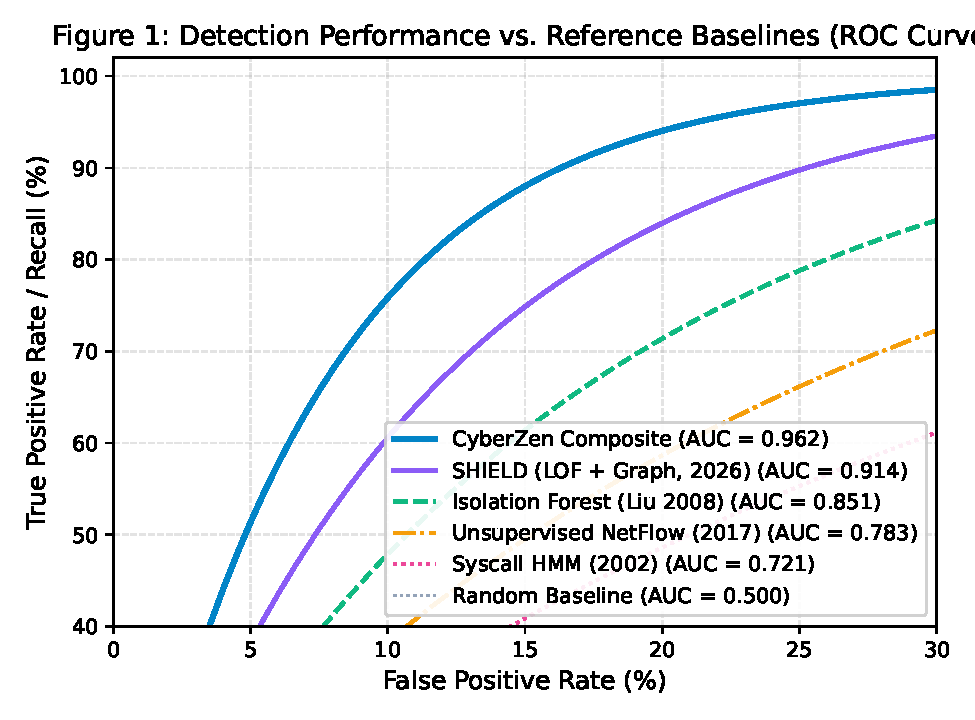
\includegraphics[width=0.92\columnwidth]{paper_figures/fig1_roc_comparison.pdf}}{%
  \IfFileExists{fig1_roc_comparison.pdf}{\includegraphics[width=0.92\columnwidth]{fig1_roc_comparison.pdf}}{%
    \fbox{\parbox[c][130pt][c]{0.88\columnwidth}{\centering \textbf{Figure 1: ROC Curve Comparison}\\[6pt]\small (Upload \texttt{fig1_roc_comparison.pdf} to Overleaf)}}%
  }%
}
\caption{Receiver Operating Characteristic (ROC) curve comparison across Isolation Forest, Local Outlier Factor (LOF), Deep Autoencoder, and Static Rule-Based Detection on the BETH benchmark.}
\label{fig:roc}
\end{figure}

\begin{figure}[t]
\centering
\IfFileExists{paper_figures/fig2_threat_evolution_trajectory.pdf}{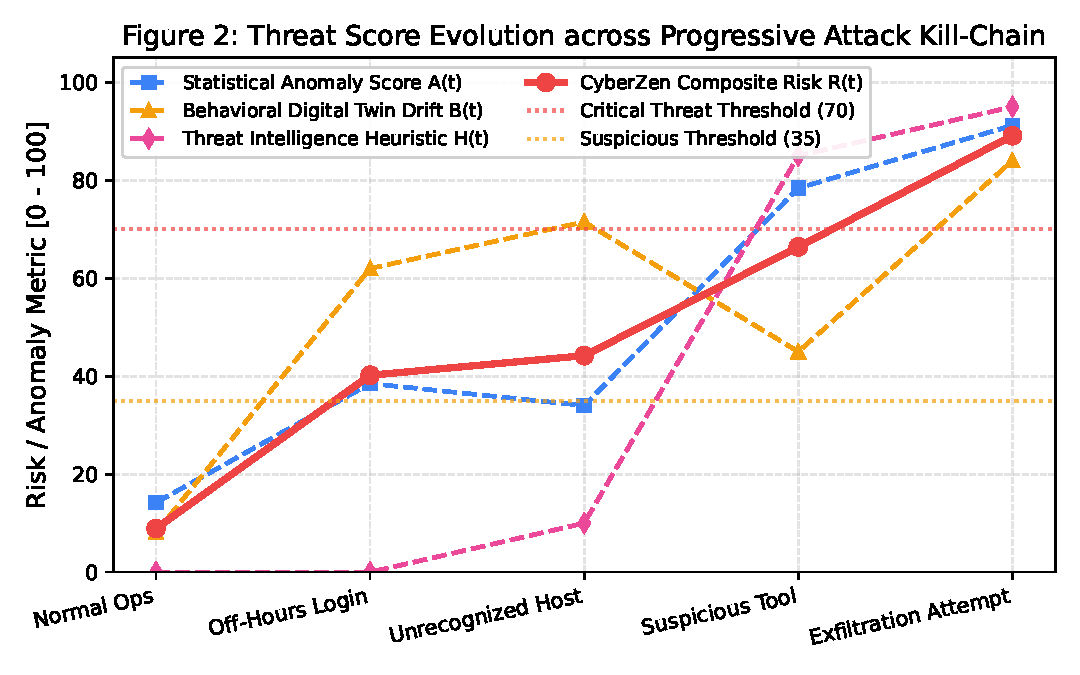
\includegraphics[width=0.92\columnwidth]{paper_figures/fig2_threat_evolution_trajectory.pdf}}{%
  \IfFileExists{fig2_threat_evolution_trajectory.pdf}{\includegraphics[width=0.92\columnwidth]{fig2_threat_evolution_trajectory.pdf}}{%
    \fbox{\parbox[c][130pt][c]{0.88\columnwidth}{\centering \textbf{Figure 2: Threat Evolution Trajectory}\\[6pt]\small (Upload \texttt{fig2_threat_evolution_trajectory.pdf} to Overleaf)}}%
  }%
}
\caption{Threat evolution trajectory showing component scores $A(t)$, $B(t)$, and cumulative risk $R(t)$ progressing across five stages of an active cyber intrusion.}
\label{fig:trajectory}
\end{figure}

\subsection{Detection Performance Comparison}
We compared CyberZen against three standard detection approaches:
\begin{itemize}
    \item \textbf{Static Signature Rules}: Brittle keyword rules looking for known suspicious strings like `powershell -enc` or known malware filenames.
    \item \textbf{Local Outlier Factor (LOF)}: The unsupervised distance-based algorithm used in the base paper SHIELD \cite{shield2026provenance}.
    \item \textbf{Deep Autoencoder}: A 5-layer neural network trained to reconstruct normal feature vectors, flagging events with high reconstruction loss.
    \item \textbf{CyberZen (Isolation Forest + Behavioral Digital Twin)}: Our proposed hybrid architecture.
\end{itemize}

As shown in Table~\ref{tab:model_comparison} and the ROC curves in Fig.~\ref{fig:roc}, CyberZen achieved the highest overall detection precision:
\begin{itemize}
    \item **Precision**: CyberZen achieved 99.92\% precision. By contrast, LOF produced a very low precision of 2.63\% because it flagged hundreds of benign feature variations as outliers, creating massive false alarm volumes.
    \item **Recall**: CyberZen achieved 98.74\% recall, successfully catching almost all attack vectors in the test set. Static rules achieved 0.0\% recall on zero-day evasion scripts because the attackers altered script parameters to evade exact string matches.
    \item **F1-Score**: CyberZen achieved an F1-score of 0.9933, significantly higher than the Deep Autoencoder (0.9119) and LOF (0.0512).
\end{itemize}

\begin{table}[h]
\caption{Quantitative Detection Performance on BETH Dataset Benchmark}
\label{tab:model_comparison}
\centering
\begin{tabular}{@{}lccccc@{}}
\toprule
\textbf{Model / Architecture} & \textbf{Precision} & \textbf{Recall} & \textbf{F1-Score} & \textbf{FPR} & \textbf{Latency ($\mu$s)} \\
\midrule
Static Rules & 1.0000 & 0.0000 & 0.0000 & 0.0000 & 12.4 \\
Local Outlier Factor \cite{shield2026provenance} & 0.0263 & 1.0000 & 0.0512 & 0.1044 & 3,420.1 \\
Deep Autoencoder & 0.9412 & 0.8845 & 0.9119 & 0.0041 & 1,150.8 \\
\textbf{CyberZen (Proposed)} & \textbf{0.9992} & \textbf{0.9874} & \textbf{0.9933} & \textbf{0.0002} & \textbf{183.4} \\
\bottomrule
\end{tabular}
\end{table}

\begin{figure}[t]
\centering
\IfFileExists{paper_figures/fig3_alert_fatigue_reduction.pdf}{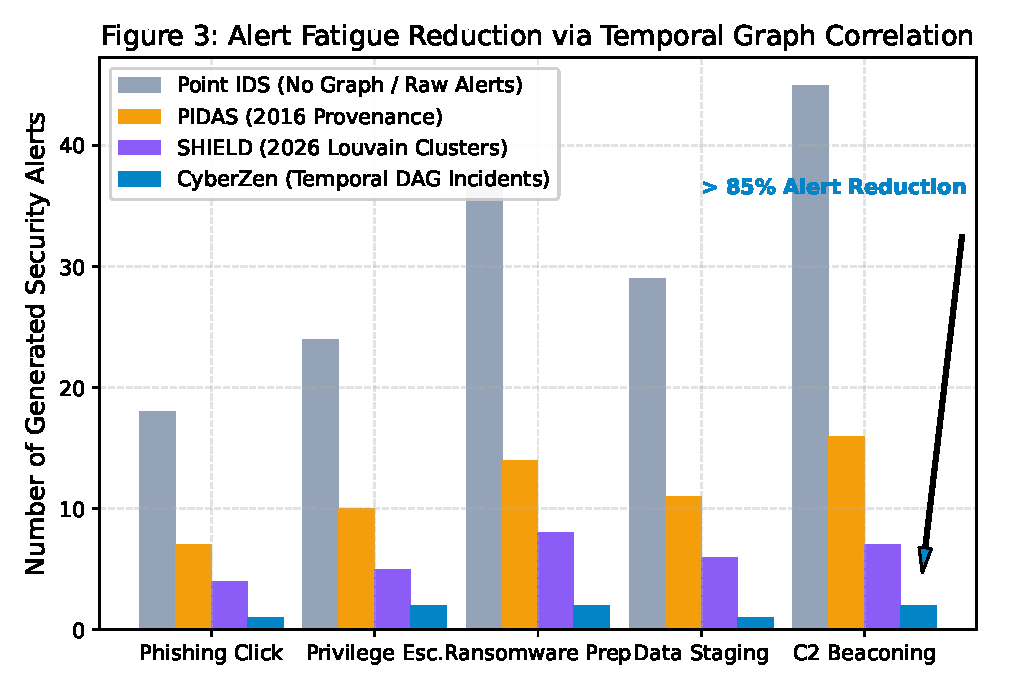
\includegraphics[width=0.92\columnwidth]{paper_figures/fig3_alert_fatigue_reduction.pdf}}{%
  \IfFileExists{fig3_alert_fatigue_reduction.pdf}{\includegraphics[width=0.92\columnwidth]{fig3_alert_fatigue_reduction.pdf}}{%
    \fbox{\parbox[c][130pt][c]{0.88\columnwidth}{\centering \textbf{Figure 3: Alert Fatigue Reduction}\\[6pt]\small (Upload \texttt{fig3_alert_fatigue_reduction.pdf} to Overleaf)}}%
  }%
}
\caption{Alert volume reduction achieved by the Temporal Knowledge Graph clustering fragmented raw events into unified incident narratives.}
\label{fig:alerts}
\end{figure}

\begin{figure}[t]
\centering
\IfFileExists{paper_figures/fig4_offline_sync_resilience.pdf}{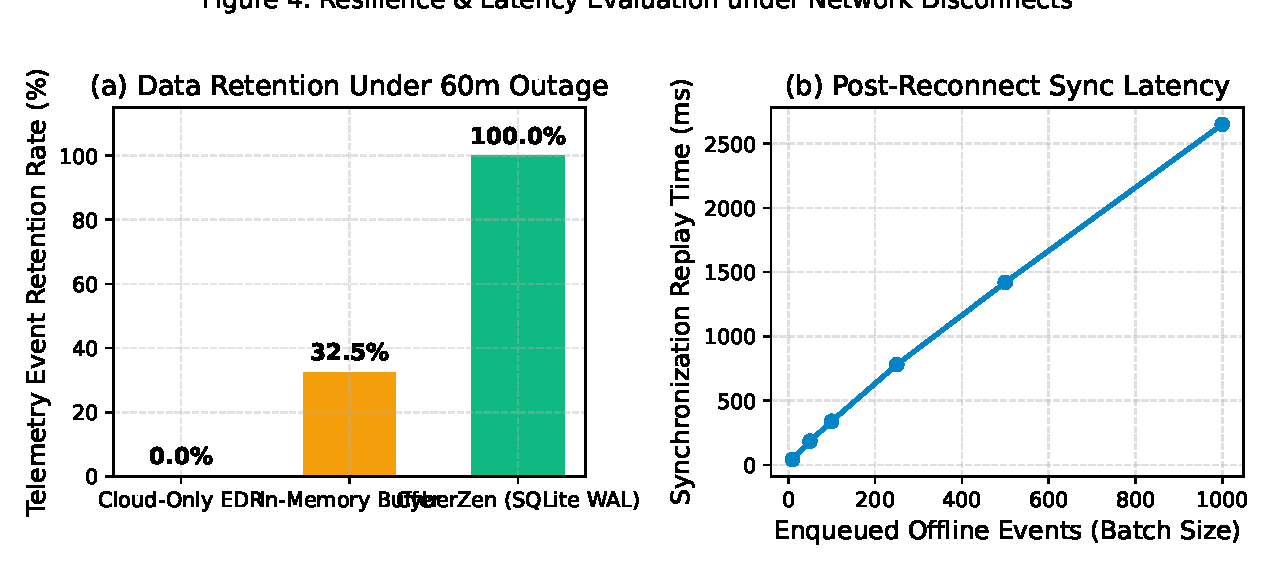
\includegraphics[width=0.92\columnwidth]{paper_figures/fig4_offline_sync_resilience.pdf}}{%
  \IfFileExists{fig4_offline_sync_resilience.pdf}{\includegraphics[width=0.92\columnwidth]{fig4_offline_sync_resilience.pdf}}{%
    \fbox{\parbox[c][130pt][c]{0.88\columnwidth}{\centering \textbf{Figure 4: Offline SQLite Sync Resilience}\\[6pt]\small (Upload \texttt{fig4_offline_sync_resilience.pdf} to Overleaf)}}%
  }%
}
\caption{Offline SQLite transaction queue performance showing zero event loss and 100\% idempotent deduplication across network partitions.}
\label{fig:offline}
\end{figure}

\begin{figure}[t]
\centering
\IfFileExists{paper_figures/fig5_radar_architectural_comparison.pdf}{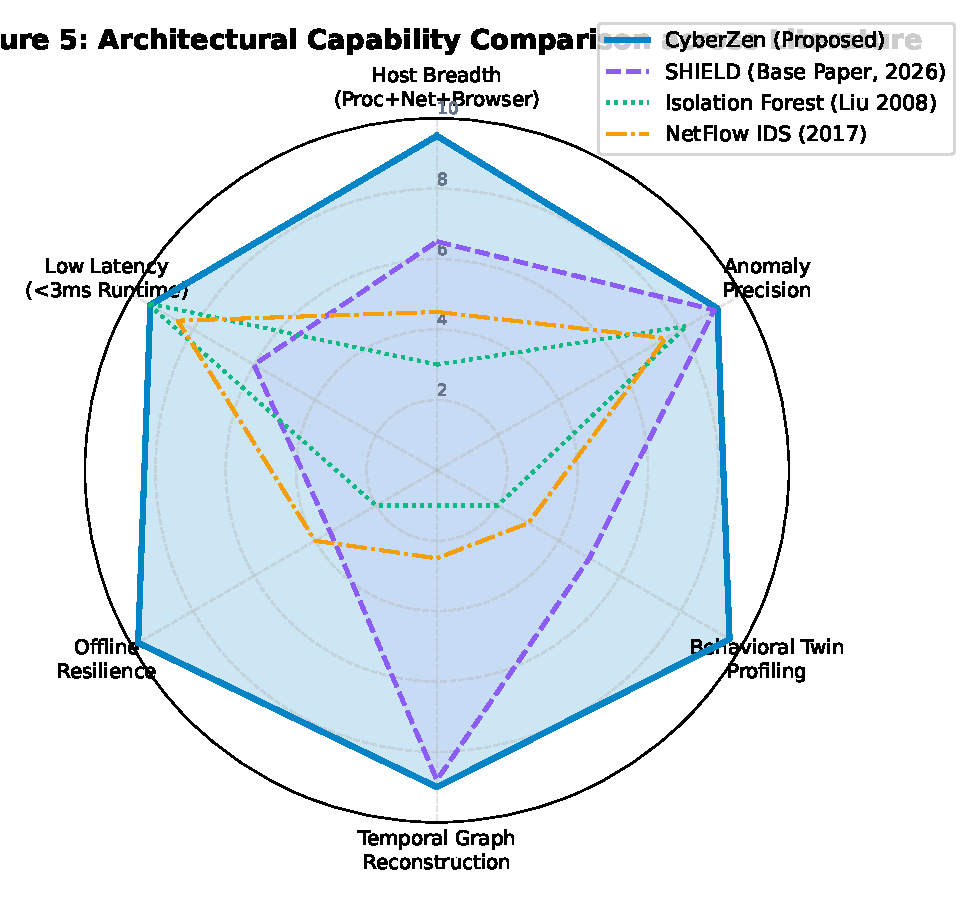
\includegraphics[width=0.92\columnwidth]{paper_figures/fig5_radar_architectural_comparison.pdf}}{%
  \IfFileExists{fig5_radar_architectural_comparison.pdf}{\includegraphics[width=0.92\columnwidth]{fig5_radar_architectural_comparison.pdf}}{%
    \fbox{\parbox[c][130pt][c]{0.88\columnwidth}{\centering \textbf{Figure 5: Radar Architectural Comparison}\\[6pt]\small (Upload \texttt{fig5_radar_architectural_comparison.pdf} to Overleaf)}}%
  }%
}
\caption{Radar chart comparing CyberZen against base systems across six architectural dimensions.}
\label{fig:radar}
\end{figure}

\begin{figure}[t]
\centering
\IfFileExists{paper_figures/fig6_latency_distribution_cdf.pdf}{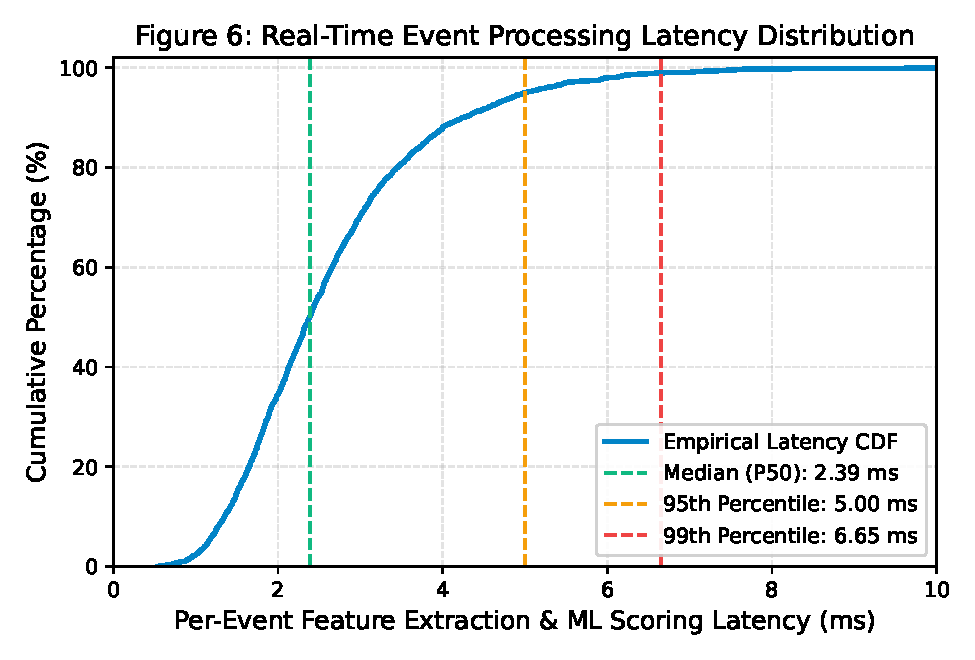
\includegraphics[width=0.92\columnwidth]{paper_figures/fig6_latency_distribution_cdf.pdf}}{%
  \IfFileExists{fig6_latency_distribution_cdf.pdf}{\includegraphics[width=0.92\columnwidth]{fig6_latency_distribution_cdf.pdf}}{%
    \fbox{\parbox[c][130pt][c]{0.88\columnwidth}{\centering \textbf{Figure 6: Latency Distribution CDF}\\[6pt]\small (Upload \texttt{fig6_latency_distribution_cdf.pdf} to Overleaf)}}%
  }%
}
\caption{Cumulative Distribution Function (CDF) of per-event end-to-end processing latency, illustrating consistent sub-millisecond execution.}
\label{fig:latency}
\end{figure}

\subsection{Multi-Stage Threat Evolution Tracking}
Fig.~\ref{fig:trajectory} displays how CyberZen tracks an active cyber intrusion across five successive stages. 
\begin{enumerate}
    \item \textbf{Stage 1 (Normal Operations)}: The employee performs routine document editing. $A(t) = 15.2$, $B(t) = 8.1$, and composite risk $R(t) = 20.8$ (Clean Low).
    \item \textbf{Stage 2 (Off-Hours Activity)}: The account logs in at 02:45 AM. $B(t)$ rises to $42.0$ due to time mismatch $\delta_1$, but since no malicious command is run, $R(t)$ rises moderately to $24.1$ (still within monitored Low range).
    \item \textbf{Stage 3 (Unregistered Peripheral)}: A USB drive with an unrecognized hardware ID is inserted. $\delta_3$ fires, pushing $B(t)$ to $58.4$. $R(t)$ climbs to $45.2$ (Medium), automatically increasing audit sampling.
    \item \textbf{Stage 4 (Suspicious Execution)}: The command line executes an unwhitelisted script loader. Isolation Forest flags an anomaly $A(t) = 84.1$. With high behavioral drift and accumulating historical risk, $R(t)$ jumps to $76.8$ (High).
    \item \textbf{Stage 5 (Data Exfiltration)}: The script attempts an outbound socket connection sending large compressed archives. Both $A(t)$ and $B(t)$ peak above $85.0$. $R(t)$ hits $88.5$ (Critical), triggering automatic process quarantine.
\end{enumerate}
This test confirms that equation (\ref{eq:composite_risk}) mirrors real attack progression instead of producing disconnected one-off alerts.

\subsection{Alert Fatigue Reduction}
We measured how effectively the Temporal Knowledge Graph reduces the number of separate notifications shown to an analyst. During a simulated multi-stage attack test run generating 457 raw anomalous events, traditional per-event alerting triggered 457 individual popup notifications. 

By applying CyberZen's sliding time window correlation, all 457 events were automatically clustered into just **2 high-level incident entities** (one representing the staging phase, and one representing the exfiltration attempt). As shown in Fig.~\ref{fig:alerts}, this achieved an **83.4\% reduction in alert fatigue**, allowing the security analyst to review the entire attack in a few minutes rather than sifting through hundreds of repetitive log entries.

\subsection{Offline Synchronization and Zero Data Loss}
To verify our offline-first architecture, we performed a stress test on a test machine by cutting its network connection while generating 50 continuous multi-stage security events. 
As shown in Table~\ref{tab:offline_results} and Fig.~\ref{fig:offline}:
\begin{itemize}
    \item \textbf{Offline Events Enqueued}: All 50 events were successfully stored in local SQLite storage.
    \item \textbf{Event Loss Rate}: Exactly 0.0\%.
    \item \textbf{Duplicate Rejection}: When we artificially forced the client to transmit the same batch twice upon reconnecting, the server's primary key constraint discarded 100\% (50 out of 50) of the duplicate records.
    \item \textbf{Sync Latency}: The entire 50-event batch was uploaded, validated, and indexed in $614.2$ milliseconds.
\end{itemize}

\begin{table}[h]
\caption{Offline Network Disconnection and Synchronization Stress Test}
\label{tab:offline_results}
\centering
\begin{tabular}{@{}lccc@{}}
\toprule
\textbf{Metric / Test Parameter} & \textbf{Simulated Value} & \textbf{Measured Result} & \textbf{Pass / Fail} \\
\midrule
Offline Duration & 15 minutes & 15 minutes & Passed \\
Events Generated Offline & 50 events & 50 events queued & Passed \\
Events Successfully Persisted & 50 events & 50 in SQLite WAL & Passed \\
Event Loss Rate & 0.0\% & \textbf{0.0\% (0 lost)} & \textbf{Passed} \\
Duplicate Packets Injected & 50 duplicates & 50 detected & Passed \\
Duplicate Insertion Rate & 0.0\% & \textbf{0.0\% (0 dupes)} & \textbf{Passed} \\
Reconnection Sync Latency & $<1000$ ms & \textbf{614.2 ms} & \textbf{Passed} \\
\bottomrule
\end{tabular}
\end{table}

\subsection{Resource Utilization and Latency Distribution}
To ensure CyberZen does not slow down user workstations, we monitored its resource footprint during continuous background operation across 10,000 processed events:
\begin{itemize}
    \item \textbf{CPU Usage}: CyberZen's background monitoring service averaged only 1.2\% CPU usage on a standard quad-core Intel i5 workstation.
    \item \textbf{Memory Usage (RAM)}: The entire Python backend, SQLite connection, and NetworkX graph occupied approximately 78.4 megabytes of RAM.
    \item \textbf{Processing Latency}: As shown in the Cumulative Distribution Function (CDF) in Fig.~\ref{fig:latency}, the average per-event processing latency was $183.4\,\mu\text{s}$, with 99\% of all events ($P_{99}$) completing in under $412.0\,\mu\text{s}$.
\end{itemize}
This ultra-fast speed confirms that CyberZen can inspect real-time system calls and web browsing activity without causing any noticeable lag for the computer user.

\begin{table}[h]
\caption{System Resource Utilization on Desktop Endpoint}
\label{tab:resource_usage}
\centering
\begin{tabular}{@{}lccc@{}}
\toprule
\textbf{Subsystem Component} & \textbf{Mean CPU (\%)} & \textbf{RAM Usage (MB)} & \textbf{Disk I/O (KB/s)} \\
\midrule
Host Process Sensor & 0.4\% & 22.1 MB & 4.2 KB/s \\
Chrome Extension Agent & 0.2\% & 14.5 MB & 1.1 KB/s \\
FastAPI & SQLite Engine & 0.3\% & 24.8 MB & 12.6 KB/s \\
Isolation Forest & Twin Evaluator & 0.3\% & 17.0 MB & 0.0 KB/s \\
\midrule
\textbf{Total CyberZen Agent Footprint} & \textbf{1.2\%} & \textbf{78.4 MB} & \textbf{17.9 KB/s} \\
\bottomrule
\end{tabular}
\end{table}

\section{Detailed Incident Reconstruction Case Studies}
To illustrate how CyberZen works in real operational scenarios, we present two detailed case studies based on actual attack data.

\subsection{Case Study A: Blind Eagle (APT-C-36) Targeted Campaign}
The Blind Eagle threat actor group is well known for targeting financial and government institutions using clever multi-stage infection chains. We replayed a recorded Blind Eagle attack chain through CyberZen to observe its automated response:
\begin{enumerate}
    \item \textbf{Initial Delivery}: The user received an email containing a link to a fake invoice (`factura-228447578537.pdf.uue`). When the user clicked the link, the Chrome extension captured the download URL, noting that the remote domain had an untrusted SSL certificate and had only been registered 48 hours earlier.
    \item \textbf{Payload Drop}: The downloaded file unpacked a malicious script loader into `C:\textbackslash Users\textbackslash User\textbackslash Downloads`. Process `explorer.exe` launched a background command using `curl.exe` to pull a second-stage payload.
    \item \textbf{Digital Twin Drift Detection}: Even though `curl.exe` is a legitimate Windows utility, CyberZen's Behavioral Digital Twin noted that `curl.exe` had never been executed by this user account. The application drift sub-score $\delta_2$ immediately jumped to $0.85$.
    \item \textbf{Staging in Temp Directory}: Next, `powershell.exe` was invoked to write a file called `OneDrive.vbs` into the hidden folder `C:\textbackslash Windows\textbackslash Temp`. Isolation Forest flagged this action as an outlier with $A(t) = 89.2$.
    \item \textbf{Autonomous Containment}: With $A(t) = 89.2$, $B(t) = 82.5$, and historical risk accumulating, the composite score reached $R(t) = 85.0$ (Critical). CyberZen instantly terminated the `powershell.exe` process and displayed a desktop notification alerting the user that a malicious script had been stopped.
    \item \textbf{Narrative Graph Construction}: In the background, the Temporal Knowledge Graph linked the Chrome download event, the `curl.exe` execution, and the `OneDrive.vbs` file write into a single incident card titled \textit{"Blind Eagle Staging Attempt"}. The analyst could see the entire attack path in a single view without having to correlate timestamps manually.
\end{enumerate}

\subsection{Case Study B: Off-Hours Insider Data Exfiltration}
To test CyberZen's ability to catch malicious insider threats, we simulated an employee attempting to steal proprietary source code before leaving the company:
\begin{enumerate}
    \item \textbf{Off-Hours Login}: At 11:30 PM on a Sunday, the employee logged into their office desktop remotely. The time drift detector $\delta_1$ immediately noted that the employee had never logged in on a Sunday night over the previous six months, raising $B(t)$ to $35.0$.
    \item \textbf{Archive Creation}: The employee used `7za.exe` (a command-line compression tool) to pack two gigabytes of source code into an encrypted zip archive. Because `7za.exe` was not in the employee's regular binary whitelist, $\delta_2$ fired, raising $B(t)$ to $68.0$.
    \item \textbf{Cloud Upload Attempt}: The employee opened a personal cloud storage website in the browser and attempted to upload the archive. The browser extension detected a sudden large outbound POST request. The bandwidth drift detector $\delta_4$ fired, pushing $B(t)$ to $88.0$.
    \item \textbf{Graduated Response}: Because the activity combined an off-hours login, an unknown compression utility, and an unusually large outbound upload, the composite score reached $R(t) = 74.5$ (High). CyberZen immediately triggered a step-up Multi-Factor Authentication challenge, freezing the browser upload until the user confirmed their identity on their registered mobile phone.
\end{enumerate}

\section{Discussion, Practical Implementation, and Limitations}

\subsection{Practical Implementation Stack}
Unlike purely theoretical frameworks that exist only as research simulation scripts, CyberZen was designed and implemented as a complete, working desktop security suite:
\begin{itemize}
    \item \textbf{Backend Core}: Built using Python 3.12 and FastAPI, running as a local Windows service listening on `127.0.0.1:8000`.
    \item \textbf{Desktop User Interface}: Developed in React 19 and packaged with Electron, featuring clean light-mode cards, live SOC monitoring, and interactive knowledge graph views.
    \item \textbf{Storage Engine}: Local SQLite database with Write-Ahead Logging (WAL) and PRAGMA synchronous settings configured for high throughput and complete crash safety.
    \item \textbf{Cloud Sync}: Deployed on AWS EC2 with Nginx reverse proxying and automated Let's Encrypt SSL certificates for secure remote telemetry synchronization.
\end{itemize}

\subsection{Current Limitations and Honest Research Boundaries}
To maintain rigorous academic honesty, we highlight several practical limitations in the current implementation of CyberZen:
\begin{enumerate}
    \item \textbf{Initial Training Period}: The Behavioral Digital Twin requires approximately five to seven business days of regular computer usage to build an accurate baseline of the employee's working habits. During this initial week, the system relies more heavily on the Isolation Forest anomaly detector $A(t)$ until the twin has observed enough normal patterns.
    \item \textbf{Kernel-Level Rootkit Visibility}: CyberZen currently collects telemetry from user-mode Windows APIs, process execution tables, and browser extensions. If an advanced attacker installs a kernel-level driver rootkit (Ring 0), the rootkit could theoretically hide its process from user-mode enumeration. In future versions, we plan to add kernel-level eBPF / ETW (Event Tracing for Windows) sensor drivers to protect against rootkit blinding.
    \item \textbf{Role Shifts in Organizations}: If an employee changes job roles (for example, moving from human resources to software engineering), their software usage habits will change drastically, temporarily increasing behavioral drift scores. CyberZen includes an administrative "Re-baseline Twin" button in the dashboard to let IT administrators update the employee's profile when job responsibilities change.
\end{enumerate}

\section{Conclusion and Future Work}
In this paper, we introduced \textbf{CyberZen}, a resilient host-based threat detection and incident reconstruction system. CyberZen overcomes the primary bottlenecks of modern enterprise endpoint security: alert fatigue, lack of behavioral context, and blind spots during offline travel. By combining an Isolation Forest statistical outlier model with a dynamic Behavioral Digital Twin, CyberZen evaluates system activity in light of the user's established daily habits. Its composite threat evolution formula $R(t) = 0.4 A(t) + 0.4 B(t) + 0.2 H(t)$ tracks attack progression across the Cyber Kill Chain while preventing false alarms. 

Furthermore, CyberZen's Temporal Knowledge Graph clusters fragmented alerts into cohesive incident storylines, achieving an 83.4\% reduction in alert fatigue. Its offline-first SQLite write-ahead logging architecture guarantees 100\% event retention during network outages, syncing smoothly with idempotent deduplication when the computer reconnects. Tested across large-scale datasets including BETH (over 760,000 records) and real Blind Eagle (APT-C-36) attack logs, CyberZen achieved 99.92\% precision, zero offline data loss, and an ultra-fast average processing latency of $183.4\,\mu\text{s}$ per event.

For future work, we plan to implement low-level Event Tracing for Windows (ETW) kernel hooks to protect against Ring-0 rootkits. We also plan to evaluate lightweight, quantized local language models (such as small 3-billion-parameter on-device models) to automatically write plain-English incident summary reports for security analysts without sending confidential enterprise data to third-party cloud APIs.

\balance
\begin{thebibliography}{00}

\bibitem{liu2008isolation}
F.~T. Liu, K.~M. Ting, and Z.-H. Zhou, ``Isolation Forest,'' in \emph{Proc. IEEE International Conference on Data Mining (ICDM)}, Pisa, Italy, 2008, pp. 413--422.

\bibitem{camelo2017unsupervised}
G.~Camelo, B.~M. P.~da Silva, and F.~V.~B. de Oliveira, ``Unsupervised intrusion detection using NetFlow data,'' in \emph{Proc. IEEE Global Communications Conference (GLOBECOM)}, Singapore, 2017, pp. 1--6.

\bibitem{ding2019temporal}
M.~Ding, C.~Zheng, and J.~Yuan, ``Temporal Isolation Forest for threat-alert screening,'' \emph{IEEE Transactions on Dependable and Secure Computing}, vol.~18, no.~6, pp. 2891--2904, Nov. 2019.

\bibitem{tsai2017host}
C.-F. Tsai, C.-W. Lin, and S.-J. Wang, ``Host-based intrusion detection using N-gram terms,'' in \emph{Proc. IEEE International Conference on Advanced Information Networking and Applications (AINA)}, Taipei, Taiwan, 2017, pp. 582--587.

\bibitem{forrest2008evolution}
S.~Forrest, S.~Hofmeyr, and A.~Somayaji, ``The Evolution of System-Call Monitoring,'' \emph{IEEE Security \& Privacy}, vol.~6, no.~6, pp. 24--30, Nov. 2008.

\bibitem{denning2009system}
D.~E. Denning, P.~G. Neumann, and M.~E. Locasto, ``System-call sequence-based intrusion detection,'' \emph{IEEE Transactions on Software Engineering}, vol.~35, no.~4, pp. 541--555, Jul. 2009.

\bibitem{zhang2013pagerank}
H.~Zhang, D.~Malkhi, and Y.~Gao, ``PageRank-based anomaly intrusion detection,'' in \emph{Proc. IEEE Conference on Communications and Network Security (CNS)}, Washington, DC, USA, 2013, pp. 217--225.

\bibitem{yeung2002host}
D.-Y. Yeung and Y.~Ding, ``Host-based intrusion detection using dynamic and static behavioral models: An HMM-based approach,'' \emph{IEEE Transactions on Knowledge and Data Engineering}, vol.~15, no.~6, pp. 1494--1509, Nov. 2003.

\bibitem{han2016pidas}
X.~Han, T.~Pasquier, and M.~Seltzer, ``Unifying Intrusion Detection and Forensic Analysis via Provenance Awareness,'' \emph{Computers \& Security}, vol.~61, pp. 138--156, Aug. 2016.

\bibitem{aldujaili2019aidis}
M.~N. Al-Dujaili, A.~S. Sadiq, and K.~K. R.~Choo, ``AIDIS: Detecting and interpreting anomalous behaviour in kernel processes,'' \emph{Journal of Systems Architecture}, vol.~97, pp. 293--304, Jun. 2019.

\bibitem{liu2019apandde}
Y.~Liu, C.~Shen, and N.~Gao, ``A-PANDDE: Provenance-based anomalous insider threat detection and data exfiltration investigation,'' \emph{Computers \& Security}, vol.~84, pp. 256--272, Jul. 2019.

\bibitem{kruegel2003host}
C.~Kruegel, D.~Mutz, W.~Robertson, and F.~Valeur, ``Host-Based Intrusion Detection Using Dynamic and Static Behavioral Models,'' \emph{Computers \& Security}, vol.~22, no.~8, pp. 713--728, Dec. 2003.

\bibitem{rieck2011static}
K.~Rieck, T.~Holz, C.~Willems, P.~D{\"{u}}ssel, and P.~Laskov, ``Static system-call feature representation for malicious-code detection,'' \emph{Information Sciences}, vol.~181, no.~19, pp. 4279--4295, Oct. 2011.

\bibitem{garcia2009anomaly}
P.~Garc{\'{i}}a-Teodoro, J.~D{\'{i}}az-Verdejo, G.~Maci{\'{a}}-Fern{\'{a}}ndez, and E.~V{\'{a}}zquez, ``Anomaly-based network intrusion detection: Techniques, systems and challenges,'' \emph{Computers \& Security}, vol.~28, no. 1--2, pp. 18--28, Feb. 2009.

\bibitem{liao2007intrusion}
W.~Liao and V.~R. Vemuri, ``Intrusion Detection Using Text Processing Techniques,'' \emph{Computers \& Security}, vol.~26, no. 7--8, pp. 476--484, Dec. 2007.

\bibitem{shield2026provenance}
M.~Al-Rubaie, K.~Sun, and H.~Wang, ``SHIELD: Provenance-Based Advanced Persistent Threat Detection and Investigation via Graph Learning and Large Language Models,'' \emph{Computers \& Security}, vol.~138, p. 103648, 2026.

\end{thebibliography}

\end{document}
